\section{MEMS module}

MirrorcleTech's MEMS micromirror technology provide ultra low-power and very fast optical beam scanning in two-axes.
Gimbal-less Two-Axis Scanning Micromirror Devices based on ARI-MEMS fabrication technology are highly versatile and adaptable to various applications.  The devices deflect laser beams to optical scanning angles of up to 30$^\circ$ at high speeds in both axes. 


Schematic diagram of MEMS mirror is shown in Fig. ~\ref{fig:mems_scheme}.
Each actuator can utilize
electrostatic rotators of arbitrary length, arbitrarily stiff linkages, and arbitrarily positioned mechanical rotation
transformers. In addition, the device can have an arbitrarily large mirror diameter.

\begin{figure}[h]
\center{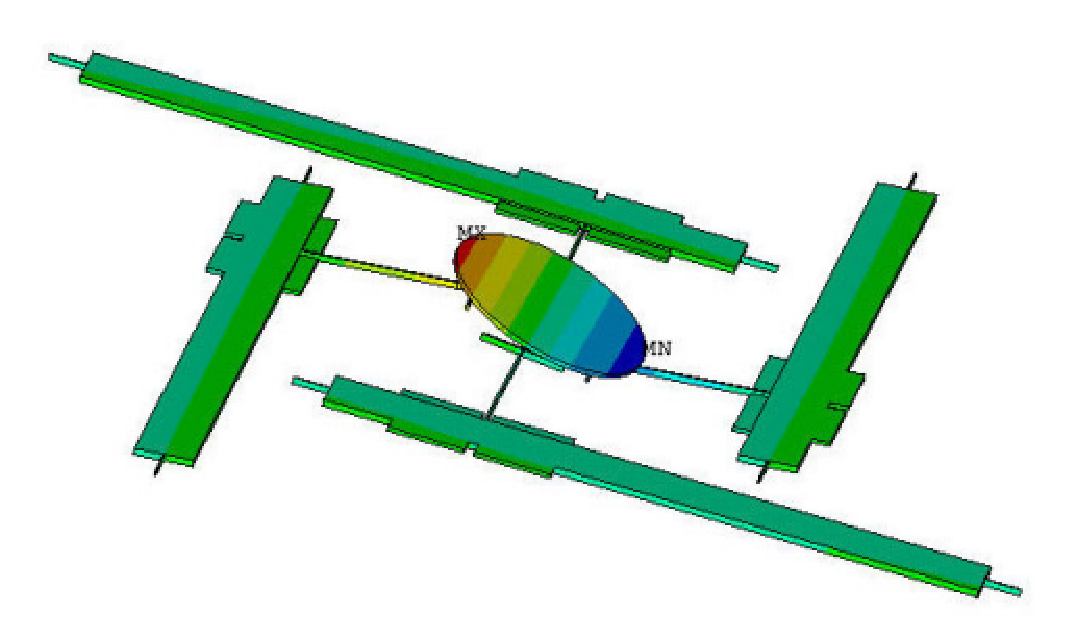
\includegraphics[width=0.55\linewidth]{mems_scheme}}
\vspace{1cm} 
\caption{Schematic diagram of an example of Mirrorcle’s proprietary gimbal-less two-axis scanning actuator based on four electrostatic bidirectional rotators connected to the central stage by special silicon linkages.}
\label{fig:mems_scheme} 
\end{figure}


Most of Mirrorcle MEMS mirrors can be operated over a very wide bandwidth from dc (they maintain position at constant voltage with nearly zero power consumption at the device) to several thousand Hertz. Such fast and broadband capability allows nearly arbitrary waveforms such as vector graphics, constant velocity line scanning, point-to-point step scanning, object tracking, etc.

\begin{figure}[h]
% \begin{floatrow}
% \ffigbox{
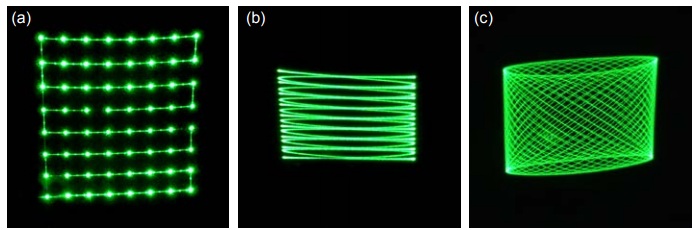
\includegraphics[width=0.85\linewidth]{mems_trajectory}

\caption{Examples of trajectories in (a) point-to-point scanning mode (quasistatic), (b) resonant
scanning mode on the x-axis (sinusoidal beam motion) and quasi-static on the y-axis (triangle wave motion), and (c) resonant scanning mode on both axes, showing a 2D resonant Lissajous pattern.}%

\label{fig:mems_trajectories} % or change caption location
\end{figure}


There is a one-to-one correspondence of actuation voltages and resulting angles: it is highly repeatable with no detectable degradation over time.  
Positional precision of mechanical tilt in open loop driving of the mirror actuatorsis at least 14 bits (16384 positions) on each axis. 
This is in great part due to the electrostatic drive methodology and singlecrystal silicon material selection.


Despite that most of the modern LiDARs are based on motor scanning, MEMS mirrors are commonly used in LiDARs too. The advantage of using MEMS mirror instead of a motor is the significant decrease of LiDAR’s size and mass in comparison. However, there are disadvantages like a small FOV (order of 20$^\circ$ instead of 360$^\circ$ in case of rotating) and a small receiver aperture, which is limited by the size of the MEMS mirror. There is trade-off between the size of the mirror, speed and scan angle. Devices with larger-diameter mirrors are correspondingly have smaller scanning angle and also scanning speed is slower due to the increased inertia, which are fouth power of radius. Thus, the scanning speed reduces quadratically with increase of mirror size.
The bonded mirrors methodology allows to select the size, as well as the geometry of mirrors for each individual application, in order to optimize the trade-offs between speed, beam size, and scan angle.


To operate MEMS mirror the driver is needed.
Digital Input MEMS Driver - PicoAmp 5.X, suggected by Mirrocle, was signigicatly redesigned, changing the size more than 2 times.
It has low voltage supply and low power consumption (<100mW).
There are 4 unipolar analog outputs ~0V-200V (X+, X-, Y-, Y+), which are used for the control of MEMS mirror via SPI commands to 16-bit DAC.
There are also ability to set any cut-off frequency for Embedded Bessel low pass filter by providing external clock signal.


\begin{figure}[H]
\center{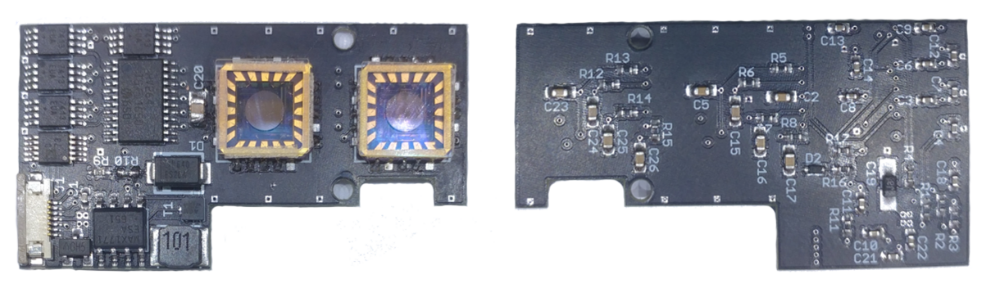
\includegraphics[width=0.7\linewidth]{MEMS_PCB}}
\caption{Upper and lower side of MEMS PCB.}
\label{fig:MEMS_PCB}
\end{figure}



For our purpose the MEMS with 3.6 mm diameter was chosen.
Already attached to the MEMS driver board the mirror is shown in the figure 
~\ref{fig:MEMS_PCB}.
The MEMS mirror characteristic are presented in table \ref{tbl:mems_characteristics}.
Important to note, that optical deflection angle by X-axis will be twice bigger.

\vspace{1cm}

\noindent%
\begin{minipage}[H]{0.5\linewidth}
This diameter of selected MEMS mirror is good enough to make possible good collimation of laser beam. The scanning FOV will be 25$^\circ$ x 13$^\circ$. The resonant frequency is enough to perform scanning at 12 FPS with 8 lines (Fig. ~\ref{fig:mems_trajectories} a)). 


\end{minipage}
\hfill
\begin{minipage}[h]{0.48\linewidth}
\begin{figure}[H]


\begin{tabular}{|M{3cm}|M{3cm}|}
\hline
Diameter: & \textbf{3.6 mm} \\  \hline
Scanning angle - X axis: & \textbf{6.6$\pmb{{^\circ}}$}  \\ \hline
Scanning angle - Y axis: & \textbf{6.5$\pmb{{^\circ}}$} \\  \hline
Resonant frequency - X axis: & \textbf{303 Hz} \\  \hline
Resonant frequency - Y axis: & \textbf{300 Hz} \\  \hline
\end{tabular}
\caption{Mirocle's MEMS mirror characteristics}
\label{tbl:mems_characteristics}

\end{figure}
\end{minipage}
\vspace{1cm}

% \begin{figure}[h]
% 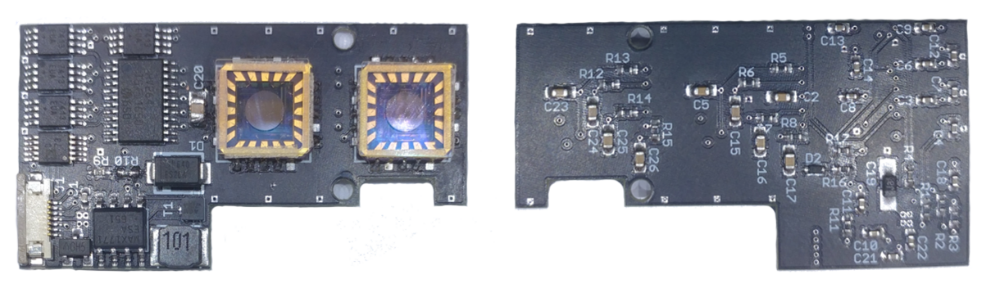
\includegraphics[width=0.65\linewidth]{MEMS_PCB}
%   \caption{By technical reasons, we used configuration with 2-MEMS (need replace by 1).}
% \label{fig:MEMS_PCB} % or change caption location
% \end{figure}

% A number of resonant-type scanning MEMS mirror designs is also offered for video projection and high rate imaging at e.g. 48000 lines/s. 

% High Speed Point-To-Point Optical Beam Scanning 
% The major advantage of our proprietary gimbal-less design is the capability to scan optical beams at equally high speeds in both axes. A typical device with a 0.8 mm diameter-sized micromirror achieves angular beam scanning of up to 500 rad/s and has first resonant frequency in both axes at approximately 4 kHz. Large angle step response settling times of <100 us have been demonstrated on devices with micromirrors up to 0.8 mm in diameter. Devices with 2.0mm diameter mirrors can achieve large angle step settling times of <1ms, with first resonance of approximately 1.3 kHz.
% SPEED VS. MIRROR SIZE TRADE-OFF










% \begin{figure}[H]
% \begin{minipage}[h]{0.52\linewidth}

% \center{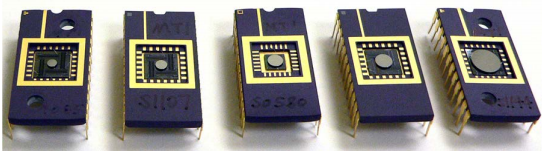
\includegraphics[width=0.55\linewidth]{mems}}
% \vspace{1cm} 
% \caption{Various MEMS actuators with bonded mirrors of different sizes. Diameters from left to right: 2.0mm, 2.4mm, 3.0mm, 3.6mm, 6.4mm in a DIP24 package}
% \label{fig:mems_scheme} 


% \end{minipage}
% \hfill
% \begin{minipage}[h]{0.45\linewidth}
% \center{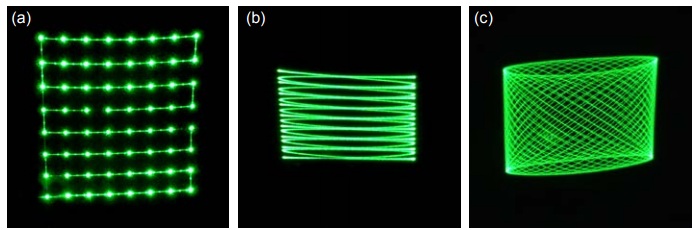
\includegraphics[height=3.05cm, width=1\linewidth]{mems_trajectory}} \\b)
% \end{minipage}
% \end{figure}

